\newpage
\section{Theory and Implementation}

\begin{figure}[!hrt]
  \centering
  \label{cavity_eom_pdh}
  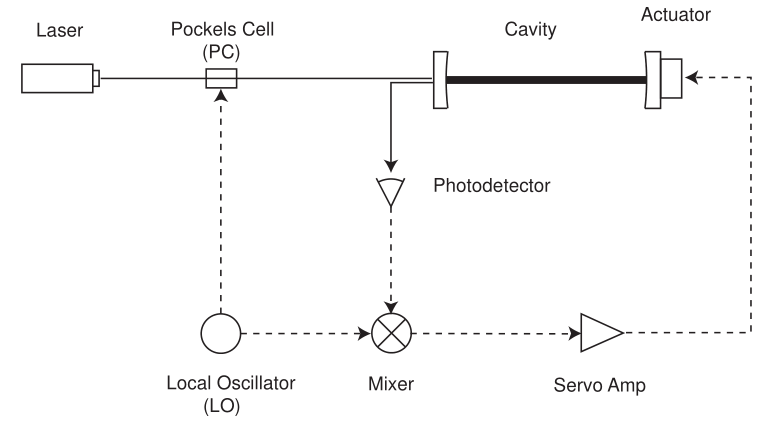
\includegraphics[scale=0.5]{cavity_eom_pdh.png}
  \caption{High level layout of PDH servo loop using an actuated cavity as
  the frequency selective element. Borrowed from \cite{black1998}}
\end{figure}


Maxwell distribution of speed in z-axis only:
\begin{gather}
  \rho(v_z) = \sqrt{\frac{m}{2\pi k_B T}} e^{\frac{-m v_z^2}{2k_B T}}
\end{gather}

Lorentzian absorption feature, with compensation for doppler shifting:
\begin{gather}
  F(\nu, v_z) = \frac{\Gamma / 2 \pi}{(\nu - \nu_0 + \nu_0 v / c)^2 +
  \Gamma^2 / 4}
\end{gather}

"Optical Depth":
\begin{gather}
  \tau(\nu) = \int_{-\infty}^\infty F(\nu, v_z) \rho(v_z) dv_z
\end{gather}

Transmission ratio:
\begin{gather}
  T(\nu) = e^{-\tau(\nu)}
\end{gather}

Terms correcting for accessible population due to pump laser:
\begin{gather}
  S(I_p, \nu) =
\end{gather}
corrected optical depth:
\begin{gather}
  \tau(\nu) = \int_{-\infty}^\infty S(I_p, \nu) F(\nu, v_z) \rho(v_z) dv_z
\end{gather}